% !TEX program = lualatex
% 解説: "How Bregman Divergences Shape Shampoo" (arXiv:2610.08534)
% ビルド: latexmk -lualatex main.tex
\documentclass[a4paper,11pt]{ltjsarticle}

\usepackage{luatexja}
\usepackage{amsmath,amssymb,amsthm,mathtools}
\usepackage{bm}
\usepackage{booktabs}
\usepackage{array}
\usepackage{multirow}
\usepackage{enumitem}
\usepackage{tikz}
\usetikzlibrary{arrows.meta,positioning,calc,decorations.pathreplacing,shapes.geometric}
\usepackage{pgfplots}
\pgfplotsset{compat=1.18}
\usepgfplotslibrary{groupplots}
\usepackage[most]{tcolorbox}
\usepackage[margin=25mm]{geometry}
\usepackage{xcolor}
\usepackage[hidelinks]{hyperref}

% ---------- 色 ----------
\definecolor{cF}{HTML}{D62728}
\definecolor{cVN}{HTML}{FF7F0E}
\definecolor{cSQ}{HTML}{2CA02C}
\definecolor{cKL}{HTML}{1F77B4}

% ---------- 定理環境 ----------
\theoremstyle{definition}
\newtheorem{definition}{定義}[section]
\newtheorem{example}[definition]{例}
\newtheorem{remark}[definition]{注意}
\theoremstyle{plain}
\newtheorem{proposition}[definition]{命題}
\newtheorem{lemma}[definition]{補題}
\renewcommand{\proofname}{証明}

% ---------- 囲み ----------
\newtcolorbox{pointbox}[1][]{enhanced,breakable,colback=blue!3,colframe=blue!50!black,
  fonttitle=\bfseries,title={#1},left=2mm,right=2mm,top=1mm,bottom=1mm}
\newtcolorbox{intuitionbox}[1][直観]{enhanced,breakable,colback=green!3,colframe=green!40!black,
  fonttitle=\bfseries,title={#1},left=2mm,right=2mm,top=1mm,bottom=1mm}
\newtcolorbox{cautionbox}[1][注意]{enhanced,breakable,colback=orange!4,colframe=orange!70!black,
  fonttitle=\bfseries,title={#1},left=2mm,right=2mm,top=1mm,bottom=1mm}

% ---------- 記号 ----------
\newcommand{\R}{\mathbb{R}}
\newcommand{\E}{\mathbb{E}}
\newcommand{\Spd}[1]{\mathbb{S}^{#1}_{++}}
\DeclareMathOperator{\Tr}{Tr}
\DeclareMathOperator{\vecop}{vec}
\DeclareMathOperator{\diag}{diag}
\DeclareMathOperator{\Var}{Var}
\newcommand{\reff}{r_{\mathrm{eff}}}
\newcommand{\ip}[2]{\langle #1,#2\rangle}
\newcommand{\norm}[1]{\lVert #1\rVert}
\newcommand{\Fro}{\mathrm{F}}
\newcommand{\T}{^{\top}}

\title{\textbf{解説：ブレグマン・ダイバージェンスは Shampoo をどう形作るか}\\[2mm]
\large Liu, Zhou, Zhao, Zhang, Kong, Dangel, Lin,\\
``How Bregman Divergences Shape Shampoo'' (arXiv:2610.08534, 2026) を大学生向けに読み解く}
\author{解説ノート}
\date{2026年10月}

\begin{document}
\maketitle

\begin{abstract}
ニューラルネットワークの最適化手法 Shampoo は、勾配の「二次モーメント行列」を
2つの小さな行列のクロネッカー積で近似し、その逆平方根で勾配を変換（前処理）する手法である。
近年、この近似を「行列どうしの距離（ダイバージェンス）を最小化する問題」とみなすことで、
F-Shampoo・VN-Shampoo・KL-Shampoo という変種が導かれた。
ところが、これらは実際の学習で性能が大きく異なり、その理由は分かっていなかった。
本稿で解説する論文は、(i) これらの変種を「トレース冪ブレグマン族」という一つの族にまとめ、
新たに PSGD と対応する SQ-Shampoo を加え、
(ii) 族の指数 $q$ が「どの固有値を重視するか」と「過大推定と過小推定のどちらを嫌うか」を決めることを示し、
(iii) 有限個の勾配から推定した二次モーメントは小さい固有値を系統的に過小評価すること、
(iv) $q$ が小さいほどクロネッカー因子の推定が安定することを示した。
これらを組み合わせると、$q$ の小さい KL と SQ が過小推定を補正し、
GPT-2 の事前学習でも F・VN より良い結果になることが説明できる。
本稿では、線形代数・最適化・統計の前提知識から丁寧に説明した上で、論文の主張と証明の要点を追う。
\end{abstract}

\tableofcontents
\clearpage

%==================================================================
\section{はじめに：この論文は何を問うているのか}
%==================================================================

深層学習のモデルは、損失関数 $\mathcal{L}(\theta)$ を小さくするようにパラメータ $\theta$ を少しずつ動かして学習する。
最も基本的な方法は確率的勾配降下法（SGD）だが、現在の大規模言語モデル（LLM）の学習では
Adam（AdamW）が標準的に使われ、さらに近年は Shampoo、SOAP、Muon、PSGD といった
「行列構造を利用する」最適化手法が注目されている。
特に Shampoo は、最適化手法のベンチマーク AlgoPerf で好成績を収めたことで一躍有名になった。

では、Shampoo は\emph{なぜ}うまくいくのか。
この問いに答えようとする研究が近年いくつも現れた。そのうちの一つの有力な見方（Lin et al., 2026）が
\begin{quote}
Shampoo は、勾配の二次モーメント行列 $C$ を、クロネッカー積 $L\otimes R$ で
\emph{ある種の距離を最小化するように}近似している
\end{quote}
というものである。「ある種の距離」としてフロベニウス距離・フォン・ノイマン・ダイバージェンス・KL ダイバージェンスを選ぶと、それぞれ
F-Shampoo、VN-Shampoo、KL-Shampoo という変種が得られる。
特に KL-Shampoo は LLM の事前学習で強い性能を示すことが報告されている。

しかし、\textbf{どの距離を選ぶとなぜ性能が変わるのか}は分かっていなかった。
本論文の中心的な問いはまさにこれである。

\begin{pointbox}[論文の中心的な問い]
異なるダイバージェンス（距離の測り方）を目的関数に選ぶと、\emph{どのように}、そして\emph{なぜ}学習性能が変わるのか？
\end{pointbox}

論文はこの問いを次の3つに分解する。
\begin{description}[leftmargin=3em]
  \item[(Q1)] ダイバージェンスの選び方は、近似誤差（どこをどれだけ間違えるか）をどう決めるか？
  \item[(Q2)] 有限個のサンプルしかないことは、クロネッカー近似にどう影響するか？
  \item[(Q3)] ダイバージェンスの選択と有限サンプルの効果は、組み合わさって前処理にどう影響するか？
\end{description}

結論を先に言えば、次のようになる。
\begin{itemize}
  \item 4つのダイバージェンス（F, VN, SQ, KL）は、指数 $q = 2, 1, 1/2, 0$ をもつ一つの族にまとまる。
  \item $q$ が小さいほど、(a) 小さい固有値（スペクトルの「裾」）にも重みを置き、
        (b) 固有値の\emph{過小推定}を強く嫌い、
        (c) 少ないサンプルからでも因子を安定に推定できる。
  \item 実データの勾配では、標本から作った二次モーメントは小さい固有値を\emph{過小評価}している。
        逆平方根をとる前処理では、過小評価は「その方向の歩幅が大きくなりすぎる」ことを意味する。
  \item したがって $q$ の小さい KL と SQ は、この過小評価を自然に打ち消し、より良い前処理になる。
        実際 GPT-2 の学習で、KL と SQ は F と VN より低い検証損失を達成した。
\end{itemize}

本稿の構成は以下の通りである。
第\ref{sec:prereq-la}節〜第\ref{sec:prereq-shampoo}節で前提知識（線形代数、前処理付き最適化、統計、ブレグマン・ダイバージェンス、Shampoo と PSGD）を説明する。
第\ref{sec:family}節以降が論文の内容の解説である。前提知識に自信のある読者は第\ref{sec:family}節から読んでもよい。

\begin{figure}[t]
\centering
\begin{tikzpicture}[
  box/.style={draw,rounded corners,align=center,minimum width=3.6cm,minimum height=1.1cm,fill=#1!8},
  arr/.style={-{Stealth[length=3mm]},thick}]
\node[box=blue] (q1) at (0,0) {\textbf{Q1} 近似誤差の配分\\{\small 第\ref{sec:family},\ref{sec:allocation}節}};
\node[box=orange] (q2a) at (5.2,0.9) {\textbf{Q2a} 目標 $C$ 自体の偏り\\{\small 第\ref{sec:reliability}節}};
\node[box=orange] (q2b) at (5.2,-0.9) {\textbf{Q2b} 因子推定のばらつき\\{\small 第\ref{sec:stability}節}};
\node[box=green] (q3) at (10.2,0) {\textbf{Q3} 前処理のゲイン\\{\small 第\ref{sec:precond}節}};
\node[box=red] (gpt) at (10.2,-2.4) {GPT-2 学習\\{\small 第\ref{sec:gpt2}節}};
\draw[arr] (q1) -- (q3);
\draw[arr] (q2a) -- (q3);
\draw[arr] (q2b) -- (q3);
\draw[arr] (q3) -- (gpt);
\end{tikzpicture}
\caption{論文の論理構成。Q1 と Q2 の結果を合わせて Q3（前処理の質）を説明し、最後に実際の学習で検証する。}
\end{figure}

%==================================================================
\section{前提知識1：線形代数}\label{sec:prereq-la}
%==================================================================

この論文は行列の言葉で書かれている。ここでは必要な道具を一通り揃える。

\subsection{対称行列・固有値分解・正定値行列}

$d\times d$ の実行列 $M$ が $M\T = M$ を満たすとき\textbf{対称行列}という。
対称行列は必ず次のように\textbf{固有値分解}できる（スペクトル定理）：
\begin{equation}
  M = U\Lambda U\T = \sum_{i=1}^d \mu_i\, u_i u_i\T,\qquad
  U = [u_1,\dots,u_d],\ \ \Lambda = \diag(\mu_1,\dots,\mu_d).
\end{equation}
ここで $U$ は直交行列（$U\T U = I$）で、列ベクトル $u_i$ は互いに直交する長さ1の\textbf{固有ベクトル}、
$\mu_i$ は対応する\textbf{固有値}である。$M u_i = \mu_i u_i$ が成り立つ。
固有値の集まり $\{\mu_i\}$ を $M$ の\textbf{スペクトル}と呼ぶ。本稿では固有値は大きい順に並べる。
大きい固有値に対応する方向を「先頭（leading）方向」、小さい固有値の方向を「裾（tail）」と呼ぶ。

\begin{intuitionbox}
対称行列 $M$ は「空間を、互いに直交する $d$ 個の方向 $u_i$ に沿って、それぞれ $\mu_i$ 倍に伸縮する変換」である。
固有値分解は、その方向と倍率を取り出す操作と思えばよい。
\end{intuitionbox}

すべての固有値が正（$\mu_i>0$）の対称行列を\textbf{正定値行列}（SPD: symmetric positive definite）という。
$d\times d$ の正定値行列全体を $\Spd{d}$ と書く。正定値であることは、任意の $x\neq 0$ に対して
$x\T M x > 0$ であることと同値である。共分散行列や二次モーメント行列は（退化していなければ）正定値である。

$x\T M x$ という量は今後何度も現れる。長さ1のベクトル $u$ について $u\T M u$ を「方向 $u$ に沿った $M$ の大きさ（スケール）」と呼ぶ。
$u$ が固有ベクトル $u_i$ なら $u_i\T M u_i = \mu_i$ である。

\subsection{行列関数：行列の平方根・逆平方根・対数}

スカラー関数 $f$ を正定値行列に適用するときは、\emph{固有値にだけ}作用させる：
\begin{equation}
  f(M) := U\,\diag\bigl(f(\mu_1),\dots,f(\mu_d)\bigr)\,U\T.
\end{equation}
たとえば
\begin{itemize}
  \item $M^{1/2} = U\diag(\sqrt{\mu_i})U\T$（行列の平方根。$M^{1/2}M^{1/2}=M$）
  \item $M^{-1/2} = U\diag(1/\sqrt{\mu_i})U\T$（逆平方根）
  \item $\log M = U\diag(\log\mu_i)U\T$（行列対数）
  \item $M^q = U\diag(\mu_i^q)U\T$（一般の冪）
\end{itemize}
である。逆平方根 $M^{-1/2}$ は「方向 $u_i$ を $1/\sqrt{\mu_i}$ 倍する」変換なので、
\textbf{固有値が小さい方向ほど大きく引き伸ばす}。この性質が論文全体の鍵になる。

\subsection{トレース・フロベニウス内積・行列式}

\textbf{トレース} $\Tr(M) = \sum_i M_{ii}$ は対角成分の和で、固有値の和 $\sum_i\mu_i$ にも等しい。
重要な性質は\textbf{巡回性} $\Tr(ABC) = \Tr(BCA) = \Tr(CAB)$ である。

行列どうしの\textbf{フロベニウス内積}は $\ip{A}{B}_\Fro = \Tr(A\T B) = \sum_{ij}A_{ij}B_{ij}$、
\textbf{フロベニウスノルム}は $\norm{A}_\Fro = \sqrt{\ip{A}{A}_\Fro}$ で定義される。
これは行列を長いベクトルとみなしたときの普通の内積・長さである。

\textbf{行列式}は固有値の積 $\det M = \prod_i\mu_i$ であり、$\log\det M = \sum_i\log\mu_i = \Tr(\log M)$ が成り立つ。

\subsection{ベクトル化とクロネッカー積}\label{sec:kron}

ニューラルネットの全結合層の重みは行列 $\Theta\in\R^{m\times n}$ であり、その勾配 $G$ も $m\times n$ 行列である。
行列をベクトルに並べ直す操作を\textbf{ベクトル化}という。本論文では行ごとに並べる（row-wise）：
\[
  G = \begin{pmatrix} a & b\\ c & e\end{pmatrix}
  \ \Longrightarrow\ 
  g = \vecop(G) = (a,b,c,e)\T \in \R^{mn}.
\]

$A\in\R^{m\times m}$, $B\in\R^{n\times n}$ の\textbf{クロネッカー積} $A\otimes B$ は、$A$ の各成分に $B$ 全体を掛けて並べた $mn\times mn$ 行列である：
\[
  A\otimes B = \begin{pmatrix} A_{11}B & \cdots & A_{1m}B\\ \vdots & \ddots & \vdots\\ A_{m1}B & \cdots & A_{mm}B\end{pmatrix}.
\]
クロネッカー積は次の便利な性質をもつ（$L, R$ は正定値とする）。
\begin{enumerate}[label=(K\arabic*)]
  \item $(A\otimes B)(C\otimes D) = (AC)\otimes(BD)$。特に $(L\otimes R)^{-1} = L^{-1}\otimes R^{-1}$、$(L\otimes R)^{p} = L^p\otimes R^p$。
  \item 行ごとのベクトル化について $\vecop(AGB) = (A\otimes B\T)\vecop(G)$。
  \item $L$ の固有値を $\ell_a$、$R$ の固有値を $\rho_b$ とすると、$L\otimes R$ の固有値は\emph{すべての積} $\ell_a\rho_b$（$mn$ 個）で、固有ベクトルは $v_{L,a}\otimes v_{R,b}$。
  \item $\Tr(L\otimes R) = \Tr(L)\Tr(R)$、$\log\det(L\otimes R) = n\log\det L + m\log\det R$、
        $\log(L\otimes R) = \log L\otimes I_n + I_m\otimes\log R$。
\end{enumerate}
(K1) と (K2) を合わせると、Shampoo の計算の核心である次の等式が得られる：
\begin{equation}\label{eq:kron-precond}
  (L\otimes R)^{-1/2}\,\vecop(G) = (L^{-1/2}\otimes R^{-1/2})\vecop(G) = \vecop\bigl(L^{-1/2}\,G\,R^{-1/2}\bigr).
\end{equation}
左辺は $mn\times mn$ という巨大な行列（$m=n=1024$ なら約 $10^{12}$ 成分）を扱う計算に見えるが、
右辺は $m\times m$ と $n\times n$ の小さな行列を左右から掛けるだけで済む。これがクロネッカー近似の計算上の利点である。

\subsection{有効ランク}

正定値行列 $A$ の\textbf{有効ランク}（effective rank）を
\begin{equation}
  \reff(A) := \frac{\Tr(A)^2}{\Tr(A^2)} = \frac{(\sum_i \alpha_i)^2}{\sum_i \alpha_i^2}\qquad(\alpha_i\text{ は }A\text{ の固有値})
\end{equation}
と定める。すべての固有値が等しければ $\reff = d$（全方向が同じくらい効いている）、
一つの固有値だけが飛び抜けて大きければ $\reff\approx 1$（実質1方向しかない）となる。
「実質的に何個の方向が効いているか」を測る量である。これは第\ref{sec:stability}節で重要になる。

%==================================================================
\section{前提知識2：最適化と前処理}\label{sec:prereq-opt}
%==================================================================

\subsection{勾配降下法と確率的勾配}

勾配降下法は $\theta_{t+1} = \theta_t - \eta\nabla\mathcal{L}(\theta_t)$ で更新する（$\eta$ は学習率）。
深層学習では全データでの勾配を毎回計算するのは高価なので、ミニバッチ（データの一部）で計算した
\textbf{確率的勾配} $g_t$ を使う。$g_t$ は真の勾配の周りでランダムにばらつく。

\subsection{なぜ前処理が必要か：細長い谷}

2変数の二次関数 $\mathcal{L}(x,y) = \frac12(100x^2 + y^2)$ を考える。等高線は $x$ 方向に潰れた細長い楕円になる。
勾配は $(100x, y)$ なので、$x$ 方向の勾配は大きく $y$ 方向は小さい。
学習率を $x$ 方向に合わせて小さくすると $y$ 方向がほとんど進まず、
$y$ 方向に合わせて大きくすると $x$ 方向で振動・発散する。
曲率の比（ここでは $100$）を\textbf{条件数}といい、これが大きいと勾配降下は遅い。

この問題の解決法は、勾配に行列 $P$ を掛けて $\theta_{t+1} = \theta_t - \eta P g_t$ とすることである。
この $P$ を\textbf{前処理行列}（preconditioner）という。上の例では $P = \diag(1/100, 1)$ とすれば、
両方向が同じ速さで縮む。ニュートン法はヘッセ行列の逆 $P = H^{-1}$ を使う手法とみなせる。

\begin{figure}[t]
\centering
\begin{tikzpicture}[scale=0.9]
\begin{scope}
  \foreach \s in {0.4,0.8,1.2,1.6}{\draw[gray!60] (0,0) ellipse ({2.6*\s} and {0.55*\s});}
  \draw[cF,thick,-{Stealth}] (-3.6,0.75) -- (-3.0,-0.65) -- (-2.45,0.58) -- (-1.9,-0.5) -- (-1.4,0.42) -- (-0.95,-0.33) -- (-0.55,0.24) -- (-0.2,-0.12);
  \node[below] at (0,-1.2) {\small 前処理なし：ジグザグに進む};
\end{scope}
\begin{scope}[xshift=8cm]
  \foreach \s in {0.4,0.8,1.2,1.6}{\draw[gray!60] (0,0) circle ({0.55*\s*1.6});}
  \draw[cKL,thick,-{Stealth}] (-1.25,0.75) -- (-0.05,0.03);
  \node[below] at (0,-1.6) {\small 前処理後：まっすぐ中心へ};
\end{scope}
\end{tikzpicture}
\caption{条件数の大きい二次関数での勾配降下（左）と、前処理で等高線を円に近づけた場合（右）の模式図。}
\end{figure}

\subsection{AdaGrad・Adam：勾配の大きさで割る}

ヘッセ行列は高価なので、深層学習では\textbf{勾配そのものの統計}を使う前処理が主流である。
AdaGrad や Adam は、各座標ごとに勾配の二乗の（移動）平均 $v_i$ を求めて
\[
  \theta_i \leftarrow \theta_i - \eta\,\frac{g_i}{\sqrt{v_i}+\epsilon}
\]
と更新する。これは対角行列 $P = \diag(v)^{-1/2}$ による前処理である。
勾配がよくばらつく座標は歩幅を小さく、あまり動かない座標は歩幅を大きくする。

これを座標ごとではなく行列全体に拡張したのが \textbf{full-matrix AdaGrad} で、
勾配の\textbf{二次モーメント行列}
\begin{equation}
  C := \E[g g\T]\in\Spd{mn}
\end{equation}
を使って $P = C^{-1/2}$ とする。ここで指数が $-1/2$ である理由は次のとおり。

\begin{intuitionbox}[なぜ $C^{-1/2}$ なのか：白色化]
$\E[gg\T] = C$ のとき、$\tilde g := C^{-1/2}g$ の二次モーメントは
\[
  \E[\tilde g\tilde g\T] = C^{-1/2}\,\E[gg\T]\,C^{-1/2} = C^{-1/2}CC^{-1/2} = I.
\]
つまり $C^{-1/2}$ を掛けると、勾配はすべての方向で「大きさ1」にそろう。これを\textbf{白色化}（whitening）という。
固有値 $\lambda_i$ の方向では、勾配は典型的に $\sqrt{\lambda_i}$ 程度の大きさなので、$1/\sqrt{\lambda_i}$ 倍してそろえる。
本論文ではこの倍率 $1/\sqrt{\lambda_i}$ を方向 $u_i$ の\textbf{ゲイン}（gain, 増幅率）と呼ぶ。
\end{intuitionbox}

ここで重要な警告がある。

\begin{cautionbox}[逆平方根前処理の危うさ]
ゲインは $1/\sqrt{\lambda}$ なので、\textbf{$\lambda$ を本当の値より小さく見積もると、ゲインが大きくなりすぎる}。
たとえば真の値が $10^{-6}$ の方向を $10^{-8}$ と見積もれば、ゲインは本来の10倍になる。
小さい固有値の方向の勾配は大部分がノイズであることが多く、それを過度に増幅すると学習が不安定になる。
逆に過大に見積もれば、ゲインが小さくなるだけ（その方向の学習が遅くなるだけ）で済む。
\textbf{この非対称性}が、論文の議論の出発点の一つである。
\end{cautionbox}

\subsection{なぜクロネッカー近似が必要か}

full-matrix AdaGrad は理想的だが、$C$ は $mn\times mn$ 行列である。$m=n=1024$ の層なら
$C$ は約 $10^{12}$ 個の成分をもち、保存も逆平方根の計算も不可能である。
そこで $C$ を小さな行列のクロネッカー積 $L\otimes R$（$L\in\Spd{m}$, $R\in\Spd{n}$）で近似すれば、
式 \eqref{eq:kron-precond} により $L^{-1/2}GR^{-1/2}$ を計算するだけで済む。保存すべきは $m^2+n^2$ 個の成分だけである。

ただしクロネッカー積で表せる行列は限られている。対称行列 $C$ の自由度は $mn(mn+1)/2$ だが、
$L\otimes R$ の自由度は $m(m+1)/2 + n(n+1)/2 - 1$（$L$ を $c$ 倍し $R$ を $1/c$ 倍しても積は同じなので1引く）しかない。
したがって\textbf{一般には $C$ を正確には表せず、どこかに誤差が残る}。
「どこに誤差を押し付けるか」を決めるのが、近似の良さを測る距離（ダイバージェンス）の選び方である。

%==================================================================
\section{前提知識3：統計 ― 二次モーメントと有限標本}\label{sec:prereq-stat}
%==================================================================

\subsection{二次モーメントとその推定}

確率ベクトル $g$ の二次モーメント行列 $C = \E[gg\T]$ は、平均が0なら共分散行列と一致する。
実際には期待値は計算できないので、$N$ 個の独立なサンプル $g_1,\dots,g_N$ から
\begin{equation}
  \widehat C_N = \frac1N\sum_{n=1}^N g_n g_n\T
\end{equation}
と推定する（\textbf{経験二次モーメント}）。大数の法則により $N\to\infty$ で $\widehat C_N\to C$ となるが、
有限の $N$ では誤差がある。

\subsection{高次元では標本固有値が歪む}

次元 $d$ がサンプル数 $N$ と同程度に大きいとき、$\widehat C_N$ の固有値は真の固有値から系統的にずれる。
有名な例として、真の共分散が単位行列 $C=I$（全固有値が1）の場合でも、$d/N = \gamma$ を固定して $d, N\to\infty$ とすると、
$\widehat C_N$ の固有値は区間 $[(1-\sqrt\gamma)^2, (1+\sqrt\gamma)^2]$ に広がって分布する
（\textbf{マルチェンコ＝パスツール則}）。
本論文の設定 $d = 128^2 = 16{,}384$, $N = 20{,}480$ では $\gamma = 0.8$ であり、
この区間は約 $[0.011, 3.59]$ になる。真の値はすべて1なのに、標本の最小固有値は約 $0.01$、つまり\textbf{100分の1に過小評価}される。

\subsection{選択バイアス（勝者の呪い）}

上の現象は「選択バイアス」として直観的に理解できる。

\begin{example}[サイコロの「最も出目が小さかった」サイコロ]
100個の公平なサイコロをそれぞれ5回振り、平均の出目が最も小さかったサイコロを選ぶ。
そのサイコロの平均は、たまたま小さい目が続いたために選ばれたのであり、3.5 よりずっと小さいだろう。
しかし同じサイコロをもう一度5回振れば、平均はだいたい 3.5 に戻る。
「小さく見えたから選んだ」ものは、実際には見た目ほど小さくない。
\end{example}

経験二次モーメントの\emph{小さい固有値の方向}は、「その標本ではたまたま勾配が小さかった方向」として選ばれている。
したがって独立な別のデータで測り直すと、その方向のスケールはもっと大きい。
これが論文第4.1節（本稿第\ref{sec:reliability}節）で実データについて確認される現象である。

\subsection{ホールドアウト（別データでの検証）}

選択バイアスを避ける基本的な方法は、「方向を選ぶデータ」と「その方向の大きさを測るデータ」を分けることである。
データ $s$ で固有ベクトル $u_{s,i}$ を求め、別の独立なデータ $s'$ でその方向のスケール $u_{s,i}\T C_{s'} u_{s,i}$ を測れば、
後者は選択に使っていないので偏りがない。
これは高次元共分散推定の文献（Ledoit \& Wolf, 2012）で知られた考え方で、本論文もこれを「正解の参照値」として使う。

\subsection{指数移動平均（EMA）と有効サンプルサイズ}

最適化中は勾配が次々と得られるので、二次モーメントを\textbf{指数移動平均}（EMA）で推定する：
\begin{equation}
  A_t = \beta_2 A_{t-1} + (1-\beta_2)\,\Delta_t .
\end{equation}
$k$ ステップ前の情報には重み $w_k = (1-\beta_2)\beta_2^k$ が掛かる。
重み付き平均の\textbf{有効サンプルサイズ}は $N_{\mathrm{eff}} = 1/\sum_k w_k^2$ で定義され、計算すると
\[
  \sum_{k\ge0} w_k^2 = \frac{(1-\beta_2)^2}{1-\beta_2^2} = \frac{1-\beta_2}{1+\beta_2}
  \quad\Longrightarrow\quad
  N_{\mathrm{eff}} = \frac{1+\beta_2}{1-\beta_2}.
\]
$\beta_2 = 0.95$ なら $N_{\mathrm{eff}}\approx 39$ であり、\textbf{実際の最適化ではたった40個程度の勾配で巨大な行列を推定している}ことになる。
有限標本の影響を無視できないのはこのためである。

\subsection{ガウス分布の二次形式の公式}

第\ref{sec:stability}節の証明で使う公式を準備しておく。$z\sim\mathcal N(0,I_n)$、$A$ を対称行列とすると
\begin{equation}\label{eq:gauss-quad}
  \E[z\T Az] = \Tr(A),\qquad \Var(z\T Az) = 2\Tr(A^2).
\end{equation}
\begin{proof}[略証]
$A = V\diag(\alpha_j)V\T$ と分解し $w = V\T z$ とおくと、$w\sim\mathcal N(0,I)$ で $z\T Az = \sum_j\alpha_j w_j^2$。
$w_j^2$ は独立で平均1・分散2（$\E[w^4]=3$ より）なので、平均は $\sum\alpha_j = \Tr A$、分散は $2\sum\alpha_j^2 = 2\Tr(A^2)$。
\end{proof}
また $z, z'$ が独立に $\mathcal N(0,I)$ に従うとき、$\E[(z\T Az')^2] = \E[z\T A\,\E[z'z'^\top]\,Az] = \E[z\T A^2 z] = \Tr(A^2)$ である。

%==================================================================
\section{前提知識4：ブレグマン・ダイバージェンス}\label{sec:prereq-breg}
%==================================================================

\subsection{スカラーの場合}

「近似の良さ」を測るには、2つのものの間の「ずれ」を測る量が必要である。
最も素朴なのは二乗誤差 $(x-y)^2$ だが、ほかにもいろいろな測り方がある。
それらを統一的に扱う枠組みが\textbf{ブレグマン・ダイバージェンス}である。

\begin{definition}[スカラーのブレグマン・ダイバージェンス]
狭義凸で微分可能な関数 $f:(0,\infty)\to\R$ に対して
\begin{equation}
  d_f(x, y) := f(x) - f(y) - f'(y)(x-y).
\end{equation}
\end{definition}

\begin{figure}[t]
\centering
\begin{tikzpicture}
\begin{axis}[width=8.5cm,height=5.5cm,axis lines=left,xmin=0,xmax=3.2,ymin=-0.6,ymax=4.2,
  xtick={0.8,2.6},xticklabels={$y$,$x$},ytick=\empty,xlabel={},ylabel={},clip=false]
  \addplot[very thick,black,domain=0.05:2.85,samples=100]{0.5*x^2};
  \addplot[thick,cKL,domain=0.0:3.0]{0.32+0.8*(x-0.8)};
  \draw[dashed,gray] (axis cs:0.8,-0.6) -- (axis cs:0.8,0.32);
  \draw[dashed,gray] (axis cs:2.6,-0.6) -- (axis cs:2.6,3.38);
  \fill (axis cs:0.8,0.32) circle (1.6pt);
  \fill (axis cs:2.6,3.38) circle (1.6pt);
  \fill (axis cs:2.6,1.76) circle (1.6pt);
  \draw[cF,very thick,<->] (axis cs:2.75,1.76) -- (axis cs:2.75,3.38)
     node[midway,right] {$d_f(x,y)$};
  \node[cKL,anchor=west] at (axis cs:0.1,1.25) {$y$ での接線};
  \node[anchor=west] at (axis cs:1.6,2.6) {$f$};
\end{axis}
\end{tikzpicture}
\caption{ブレグマン・ダイバージェンスの幾何学的意味。点 $y$ で引いた接線（一次近似）と、点 $x$ での $f$ の値との差（赤）が $d_f(x,y)$ である。$f$ が凸なので常に非負で、$x=y$ のときに限り0になる。}
\label{fig:bregman}
\end{figure}

図\ref{fig:bregman}のように、$d_f(x,y)$ は「$y$ での接線で $f(x)$ を予測したときの誤差」である。
$f$ が凸なら接線は常に $f$ の下にあるので $d_f\ge 0$、等号は $x=y$ のときに限る。
ただし一般に $d_f(x,y)\neq d_f(y,x)$（\textbf{非対称}）であり、厳密な意味の「距離」ではないので「ダイバージェンス」と呼ぶ。
この非対称性が論文で重要な役割を果たす。

\begin{example}
\begin{itemize}
  \item $f(x) = x^2/2$：$d_f(x,y) = \frac12(x-y)^2$（二乗誤差）。対称。
  \item $f(x) = x\log x - x$：$d_f(x,y) = x\log\frac xy - x + y$（一般化 KL ダイバージェンス）。
  \item $f(x) = -\log x$：$d_f(x,y) = \frac xy - \log\frac xy - 1$（板倉＝斎藤ダイバージェンス）。
\end{itemize}
\end{example}

\subsection{行列の場合}

行列版は、行列関数を使って $\Phi(M) := \Tr(f(M)) = \sum_i f(\mu_i)$ と定義した $\Phi$ で同じことをする。
$\Phi$ の勾配は $\nabla\Phi(M) = f'(M)$ である。

\begin{definition}[ブレグマン行列ダイバージェンス（Dhillon \& Tropp, 2008）]
$X, Y\in\Spd{d}$ に対して
\begin{equation}\label{eq:matrix-bregman}
  B_\Phi(X, Y) := \Phi(X) - \Phi(Y) - \ip{\nabla\Phi(Y)}{X-Y}_\Fro .
\end{equation}
\end{definition}
代表的な3つは次の通り。
\begin{align}
  &\text{フロベニウス (F)}: & f(x)&=\tfrac12x^2, & B_{\mathrm F}(X,Y) &= \tfrac12\norm{X-Y}_\Fro^2,\\
  &\text{フォン・ノイマン (VN)}: & f(x)&=x\log x - x, & B_{\mathrm{VN}}(X,Y) &= \Tr(X\log X - X\log Y - X + Y),\\
  &\text{KL (LogDet)}: & f(x)&=-\log x, & B_{\mathrm{KL}}(X,Y) &= \Tr(Y^{-1}X) - \log\det(Y^{-1}X) - d.
\end{align}
KL ダイバージェンスという名前は、平均0のガウス分布どうしの KL ダイバージェンスと
$B_{\mathrm{KL}}(X,Y) = 2D_{\mathrm{KL}}(\mathcal N(0,X)\,\|\,\mathcal N(0,Y))$ の関係にあることに由来する。
VN は量子情報理論のフォン・ノイマン相対エントロピーに由来する名前である。

\subsection{ブレグマン・ダイバージェンスで行列を近似する}

本論文の枠組みでは、勾配の二次モーメント $C$ を、クロネッカー積で
\begin{equation}\label{eq:bregman-kron}
  \min_{L\in\Spd{m},\,R\in\Spd{n}}\ B_\Phi(C,\ L\otimes R)
\end{equation}
と近似する。第1引数が真の値 $C$、第2引数が近似 $S = L\otimes R$ である。
ダイバージェンスは非対称なので、\emph{引数の順番}にも意味がある点に注意しよう。

%==================================================================
\section{前提知識5：Shampoo と PSGD}\label{sec:prereq-shampoo}
%==================================================================

\subsection{Shampoo}

Shampoo（Gupta et al., 2018）は、行列パラメータ $\Theta$ の勾配 $G_t$ に対して2つの統計
\begin{equation}
  L_t = \beta_2L_{t-1} + (1-\beta_2)G_tG_t\T,\qquad R_t = \beta_2R_{t-1} + (1-\beta_2)G_t\T G_t
\end{equation}
を保持し、
\begin{equation}
  \Theta_{t+1} = \Theta_t - \eta_t\,L_t^{-p}\,G_t\,R_t^{-p}
\end{equation}
で更新する。元の Shampoo は $p = 1/4$ だが、近年の実装では $p = 1/2$ を使う。
$p=1/2$ のとき、式\eqref{eq:kron-precond} より更新は $(L_t\otimes R_t)^{-1/2}g_t$ に等しく、
$L\otimes R$ を二次モーメント $C$ の近似とみなした「近似 full-matrix AdaGrad」と解釈できる。
$G G\T$ は「行どうしの相関」、$G\T G$ は「列どうしの相関」を集めた行列であり、それらの積で全体の相関を近似するという発想である。

\subsection{ダイバージェンス最小化としての Shampoo（Lin et al., 2026）}

Lin et al.\ (2026) は、式 \eqref{eq:bregman-kron} の停留条件（勾配が0になる条件）から Shampoo 型の更新則を導いた。
たとえば VN ダイバージェンスを使うと、停留条件は
\[
  L = \frac{\E[GG\T]}{\Tr(R)},\qquad R = \frac{\E[G\T G]}{\Tr(L)}
\]
となり、Shampoo の統計 $\E[GG\T]$, $\E[G\T G]$ と（正規化を除いて）同じ形になる。
フロベニウスなら F-Shampoo、KL なら KL-Shampoo が得られる。
これらは同じ問題を\emph{違う物差し}で解いたものだが、実際の性能は大きく異なる（後述の表\ref{tab:gpt2}）。
その理由を説明するのが本論文の目的である。

\subsection{PSGD}

PSGD（preconditioned SGD, Li 2018; 2019）は Shampoo とは独立に提案された手法で、
前処理行列 $P$ を次の「勾配白色化」目的関数の最小化で学習する：
\begin{equation}\label{eq:psgd}
  \min_{P\in\Spd{mn}}\ \Tr(PC) + \Tr(P^{-1}).
\end{equation}
\begin{intuitionbox}[なぜ解が $C^{-1/2}$ になるのか]
スカラーで考えると $\min_{p>0}\ pc + 1/p$ である。微分して $c - 1/p^2 = 0$ より $p = c^{-1/2}$。
行列でも同様に、唯一の解は $P = C^{-1/2}$ となる。$\Tr(PC)$ は「$P$ を大きくしすぎるな」、
$\Tr(P^{-1})$ は「$P$ を小さくしすぎるな」という2つの力の釣り合いで解が決まる。
\end{intuitionbox}
PSGD-Kron は $P = P_L\otimes P_R$ と制約して、リー群上の相対勾配法で因子を更新する。
PSGD は実験的に強い性能を示すが、なぜうまくいくかはよく分かっていなかった。
本論文は、\textbf{PSGD の目的関数がブレグマン族の新しいメンバー（SQ）に一致する}ことを示す。

%==================================================================
\section{トレース冪ブレグマン族による統一（論文第3.1節）}\label{sec:family}
%==================================================================

ここから論文の本題に入る。まず (C1) の内容、すなわち4つのダイバージェンスを一つの族にまとめる話である。

\subsection{生成関数の族}

\begin{proposition}[Shampoo と PSGD-Kron の統一；論文の命題1]\label{prop:unify}
次のスカラー関数の族を考える：
\begin{equation}\label{eq:fq}
  f_q(x) := \frac{x^q - qx + q - 1}{q(q-1)}\ \ (q\neq0,1),\qquad
  f_1(x) := x\log x - x + 1,\qquad
  f_0(x) := -\log x + x - 1 .
\end{equation}
$\Phi_q(M) := \Tr(f_q(M))$ が生成するブレグマン・ダイバージェンス $B_{\Phi_q}$ について、
\begin{itemize}
  \item $q = 2$ はフロベニウス (F)、$q\to1$ はフォン・ノイマン (VN)、$q\to0$ は KL に一致する；
  \item $q = 1/2$（\textbf{平方根, SQ}）は、$P = S^{-1/2}$ とおくと PSGD の目的関数 \eqref{eq:psgd} に、正の定数倍と定数項を除いて一致する。
\end{itemize}
さらに $S = L\otimes R$ とおくと、停留点は次の連立方程式を満たす：
\begin{equation}\label{eq:stationary}
  L = \frac{\E[G R^{q-1}G\T]}{\Tr(R^q)},\qquad R = \frac{\E[G\T L^{q-1}G]}{\Tr(L^q)} .
\end{equation}
\end{proposition}

\begin{figure}[t]
\centering
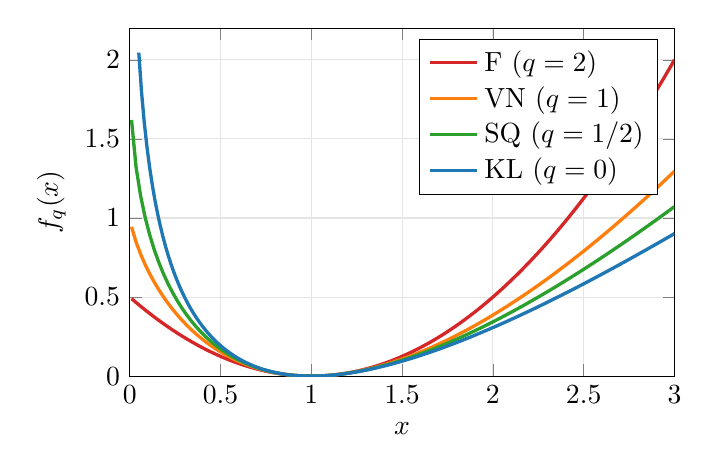
\begin{tikzpicture}
\begin{axis}[width=8.5cm,height=6cm,xmin=0,xmax=3,ymin=0,ymax=2.2,
  xlabel={$x$},ylabel={$f_q(x)$},legend pos=north east,legend cell align=left,
  grid=major,grid style={gray!20}]
  \addplot[cF,very thick,domain=0.01:3,samples=120]{(x-1)^2/2};
  \addlegendentry{F ($q=2$)}
  \addplot[cVN,very thick,domain=0.01:3,samples=120]{x*ln(x)-x+1};
  \addlegendentry{VN ($q=1$)}
  \addplot[cSQ,very thick,domain=0.01:3,samples=120]{-4*sqrt(x)+2*x+2};
  \addlegendentry{SQ ($q=1/2$)}
  \addplot[cKL,very thick,domain=0.05:3,samples=200]{-ln(x)+x-1};
  \addlegendentry{KL ($q=0$)}
\end{axis}
\end{tikzpicture}
\caption{生成関数 $f_q$。どれも $x=1$ で最小値0をとる凸関数である。$q$ が大きいほど右側（大きい $x$）で急に増え、$q$ が小さいほど左側（$x\to0$）で急に増える。KL は $x\to0$ で発散する。}
\label{fig:fq}
\end{figure}

族 \eqref{eq:fq} は、スカラーのアルファ・ベータ・ダイバージェンス（Cichocki \& Amari, 2010）の生成関数を行列に拡張したものである。
分子の $-qx+q-1$ は1次以下の項であり、ブレグマン・ダイバージェンスでは1次の項は打ち消し合うので、本質的には $x^q$（の定数倍）である。
1次の項は「$x=1$ で最小値0」となるように形を整えるためのものである。

\paragraph{極限の確認（ロピタルの定理の代わりにテイラー展開で）}
$q\to0$：$x^q = e^{q\log x} = 1 + q\log x + O(q^2)$ なので、分子は $q(\log x - x + 1) + O(q^2)$、分母は $q(q-1)\approx -q$。
したがって $f_q(x)\to -(\log x - x + 1) = -\log x + x - 1 = f_0(x)$。

$q\to1$：$q = 1+\varepsilon$ とおくと $x^q = x e^{\varepsilon\log x} = x + \varepsilon x\log x + O(\varepsilon^2)$。
分子は $\varepsilon(x\log x - x + 1) + O(\varepsilon^2)$、分母は $(1+\varepsilon)\varepsilon\approx\varepsilon$ なので $f_q\to f_1$。

$q=2$：$f_2(x) = (x^2-2x+1)/2 = (x-1)^2/2$ で、これはフロベニウス。

\paragraph{SQ が PSGD に一致すること}
$q = 1/2$ を代入すると $f_{1/2}(x) = -4\sqrt x + 2x + 2$、$f'_{1/2}(x) = 2 - 2x^{-1/2}$。
これを式 \eqref{eq:matrix-bregman} に入れて整理すると（1次の項は打ち消し合う）
\begin{equation}
  \tfrac12 B_{\Phi_{1/2}}(C, S) = \Tr(S^{1/2}) + \Tr(CS^{-1/2}) - 2\Tr(C^{1/2}).
\end{equation}
$P = S^{-1/2}$ とおけば $\Tr(S^{1/2}) = \Tr(P^{-1})$、$\Tr(CS^{-1/2}) = \Tr(PC)$ なので
\[
  \tfrac12 B_{\Phi_{1/2}}(C, S) = \Tr(PC) + \Tr(P^{-1}) - \underbrace{2\Tr(C^{1/2})}_{P\text{ に無関係}} .
\]
これは PSGD の目的関数 \eqref{eq:psgd} そのものである。
$S = L\otimes R$ なら $P = L^{-1/2}\otimes R^{-1/2}$ もクロネッカー積なので、クロネッカー制約の下でも対応が保たれる。

\begin{pointbox}[ここが新しい]
独立に開発された PSGD と Shampoo が、「ブレグマン族の $q=1/2$ のメンバー」という一つの視点でつながった。
これにより PSGD の強さも、他の Shampoo 変種と同じ枠組みで説明できるようになる。
\end{pointbox}

\subsection{停留方程式の導出（$q\neq0,1$ の場合）}

式 \eqref{eq:stationary} の導出を追ってみよう。$\nabla\Phi_q(S) = (S^{q-1} - I)/(q-1)$ をブレグマン・ダイバージェンスに代入し、
$S$ に依存する項だけを残すと
\[
  B_{\Phi_q}(C, S) = \frac1q\Tr(S^q) - \frac1{q-1}\Tr(CS^{q-1}) + \text{const}.
\]
$S = L\otimes R$ とすると、(K1)(K4) より $\Tr(S^q) = \Tr(L^q)\Tr(R^q)$。
また $C = \E[gg\T]$ と (K2) より $\Tr(CS^{q-1}) = \E[g\T(L^{q-1}\otimes R^{q-1})g] = \E\Tr(L^{q-1}GR^{q-1}G\T)$。
$R$ を固定して $A_R := \E[GR^{q-1}G\T]$, $a_R := \Tr(R^q)$ とおくと、$L$ に関する目的関数は
\[
  J_q(L;R) = \frac{a_R}{q}\Tr(L^q) - \frac{1}{q-1}\Tr(A_RL^{q-1}).
\]
$X = L^{q-1}$ と変数変換すると $L^q = X^{q/(q-1)}$ で、
\[
  \nabla_X J_q = \frac{1}{q-1}\bigl(a_R X^{1/(q-1)} - A_R\bigr) = \frac{1}{q-1}(a_RL - A_R).
\]
これを0とおくと $L = A_R/a_R$、すなわち
$L = \E[GR^{q-1}G\T]/\Tr(R^q)$ を得る（論文では $q$ への依存を明示して左辺を $L_q$ と書いている）。
$X$ について狭義凸なので、これは $R$ を固定したときの唯一の最小解である。
$q=1$（VN）と $q=0$（KL）でも、それぞれ $X = \log L$, $X = L^{-1}$ と変数変換すれば同じ形の式が得られる。

\begin{table}[t]
\centering
\caption{各変種の因子更新に使う統計量（論文の表6）。$\Psi_L$ を勾配について平均すると新しい $L$ が得られる。}
\label{tab:stats}
\renewcommand{\arraystretch}{1.3}
\begin{tabular}{lccc}
\toprule
変種 & $q$ & $\Psi_L(G;L,R)$ & $\Psi_R(G;L,R)$\\
\midrule
F-Shampoo  & 2   & $GRG\T/\Tr(R^2)$ & $G\T LG/\Tr(L^2)$\\
VN-Shampoo & 1   & $GG\T/\Tr(R)$ & $G\T G/\Tr(L)$\\
SQ-Shampoo & 1/2 & $GR^{-1/2}G\T/\Tr(R^{1/2})$ & $G\T L^{-1/2}G/\Tr(L^{1/2})$\\
KL-Shampoo & 0   & $GR^{-1}G\T/n$ & $G\T L^{-1}G/m$\\
\bottomrule
\end{tabular}
\end{table}

表\ref{tab:stats}から、各変種の違いは一目瞭然である。
$L$ を更新するとき、勾配 $G$ の列方向を $R^{q-1}$ で重み付けしている。
\begin{itemize}
  \item F（$q=2$）は $R$ を掛ける：$R$ の\emph{大きい}固有値の方向を強調する。
  \item VN（$q=1$）は何も掛けない：素の $GG\T$。Shampoo と同じ形。
  \item SQ（$q=1/2$）は $R^{-1/2}$、KL（$q=0$）は $R^{-1}$ を掛ける：反対側の因子で「白色化」してから統計を取る。
\end{itemize}
実装上は、この連立方程式を $L$ と $R$ について交互に（あるいは同時に）反復して解く（不動点反復）。
オンラインの最適化では、Lin et al.\ (2026) の方式に従い、$\Psi_L, \Psi_R$ の EMA をとり、固有基底は5ステップごとに更新する（論文付録C, Algorithm 1）。
公平な比較のため、4つの変種はすべてこの共通の実装方式で比較される。

%==================================================================
\section{近似誤差の配分（論文第3.2節）}\label{sec:allocation}
%==================================================================

第\ref{sec:prereq-opt}節で見たように、クロネッカー積は一般に $C$ を正確には表せない。
ではダイバージェンスは、残った誤差を\emph{どこに}押し付けるのか。これが Q1 である。
この性質はダイバージェンス自体の性質なので、まず一般の正定値行列 $A$（真の値）と $B$（近似）について調べる。

\subsection{固有値のずれと固有空間のずれへの分解}

\begin{proposition}[スペクトル誤差分解；論文の命題2]\label{prop:decomp}
$A = U\Lambda U\T$, $B = V\Omega V\T$ の固有値をそれぞれ $\lambda_1\ge\cdots\ge\lambda_d$, $\omega_1\ge\cdots\ge\omega_d$、
固有ベクトルの重なりを $P_{ij} := \ip{u_i}{v_j}^2$ とする。このとき
\begin{equation}
  B_\Phi(A,B) = \underbrace{\sum_{i=1}^d d_f(\lambda_i,\omega_i)}_{\text{固有値のずれ}}
  + \underbrace{\Delta_f(\Lambda,\Omega;P)}_{\text{固有空間のずれ}},\qquad \Delta_f\ge0 .
\end{equation}
ここで $\Delta_f := -\sum_{i,j}\lambda_i f'(\omega_j)(P_{ij} - \delta_{ij})$。
さらにトレース冪族 $f_q$ では、任意の $r>0$ に対して
\begin{equation}\label{eq:scaling}
  d_q(\lambda, r\lambda) = \lambda^q\, d_q(1, r),\qquad \Delta_q(r\Lambda, r\Omega; P) = r^q\,\Delta_q(\Lambda,\Omega;P).
\end{equation}
\end{proposition}

\paragraph{分解の意味}
近似が悪くなる原因は2つある。(1) 方向（固有ベクトル）は合っているが倍率（固有値）が違う、
(2) そもそも方向がずれている。命題はダイバージェンスがこの2つの和にきれいに分かれることを示す。
$P_{ij}$ は「真の $i$ 番目の方向と近似の $j$ 番目の方向がどれだけ重なっているか」で、
方向が完全に一致していれば $P = I$ となり $\Delta_f = 0$ である。

\paragraph{証明の要点}
巡回性から $\Tr(\nabla\Phi(B)A) = \Tr(f'(\Omega)Q\T\Lambda Q) = \sum_{ij}\lambda_if'(\omega_j)P_{ij}$（$Q = U\T V$）を示し、
$\sum_i\lambda_if'(\omega_i)$ を足して引けば分解が得られる。
$\Delta_f\ge0$ の証明はエレガントで、次の2つの事実を使う。
\begin{itemize}
  \item $Q$ は直交行列なので、$P_{ij} = Q_{ij}^2$ は各行・各列の和が1の\textbf{二重確率行列}である。
        バーコフ＝フォン・ノイマンの定理により、$P$ は置換行列の凸結合 $P = \sum_k\alpha_k\Pi_k$ で書ける。
  \item $\lambda_i$ は降順、$f$ は凸なので $f'$ は増加関数であり $f'(\omega_i)$ も降順。
        \textbf{並べ替え不等式}（大きいもの同士・小さいもの同士を組むと積の和が最大）より、
        どの置換 $\sigma$ についても $\sum_i\lambda_if'(\omega_{\sigma(i)})\le\sum_i\lambda_if'(\omega_i)$。
\end{itemize}
これを $\alpha_k$ で平均すれば $\sum_{ij}\lambda_if'(\omega_j)P_{ij}\le\sum_i\lambda_if'(\omega_i)$、すなわち $\Delta_f\ge0$ が得られる。

\subsection{指数 $q$ は「どの固有値を重視するか」を決める}

スケーリング則 \eqref{eq:scaling} が意味することを考えよう。
同じ「相対誤差 $r$」（たとえば2倍のずれ）でも、それが大きさ $\lambda$ の固有値で起きたときのペナルティは $\lambda^q$ に比例する。
\begin{center}
\renewcommand{\arraystretch}{1.2}
\begin{tabular}{lcccc}
\toprule
 & F & VN & SQ & KL\\\midrule
$q$ & 2 & 1 & 1/2 & 0\\
相対誤差のペナルティの重み & $\lambda^2$ & $\lambda$ & $\lambda^{1/2}$ & $1$\\
\bottomrule
\end{tabular}
\end{center}
勾配の二次モーメントの固有値は何桁にもわたって分布する（後の図で $10^{-3}$ から $10^{-9}$ 以上）。
たとえば固有値 $10^{-2}$ と $10^{-8}$ の方向で同じ2倍のずれがあったとき、
F は前者を $(10^6)^2 = 10^{12}$ 倍重く罰するので、\textbf{裾の誤差は事実上無視される}。
一方 KL は両者を同じ重さで罰する（\textbf{スケール不変}）。
同じ性質が固有空間のずれ $\Delta_q$ にも成り立つ。

\subsection{過大推定と過小推定の非対称性}

次に、真の固有値 $\lambda$ を近似 $\omega = r\lambda$ で表したときのペナルティを具体的に計算する。
一般の $q$ について $d_q(\lambda,\omega) = \frac{\lambda^q + (q-1)\omega^q - q\lambda\omega^{q-1}}{q(q-1)}$ であり、各変種では
\begin{align}
  d_{\mathrm F}(\lambda, r\lambda) &= \tfrac12\lambda^2(r-1)^2, &
  d_{\mathrm{VN}}(\lambda, r\lambda) &= \lambda\,(r - 1 - \log r),\\
  d_{\mathrm{SQ}}(\lambda, r\lambda) &= 2\lambda^{1/2}\bigl(\sqrt r + 1/\sqrt r - 2\bigr), &
  d_{\mathrm{KL}}(\lambda, r\lambda) &= \log r + 1/r - 1 .
\end{align}
$r>1$ なら近似は $r$ 倍の\textbf{過大推定}、$1/r$ に置き換えれば同じ倍率の\textbf{過小推定}である。両者を比べると
\begin{equation}\label{eq:asym}
\begin{aligned}
  d_{\mathrm F}(\lambda, r\lambda) &> d_{\mathrm F}(\lambda, \lambda/r), &
  d_{\mathrm{VN}}(\lambda, r\lambda) &> d_{\mathrm{VN}}(\lambda, \lambda/r),\\
  d_{\mathrm{SQ}}(\lambda, r\lambda) &= d_{\mathrm{SQ}}(\lambda, \lambda/r), &
  d_{\mathrm{KL}}(\lambda, r\lambda) &< d_{\mathrm{KL}}(\lambda, \lambda/r).
\end{aligned}
\end{equation}

\paragraph{確かめてみよう}
F：$(r-1)^2$ と $(1/r-1)^2 = (r-1)^2/r^2$ を比べれば、$r>1$ で前者が大きい。

SQ：$\sqrt r + 1/\sqrt r$ は $r\leftrightarrow1/r$ で不変なので完全に対称。

KL：差をとると $(\log r + 1/r - 1) - (-\log r + r - 1) = -(r - 1/r - 2\log r) =: -h(r)$。
$h(1) = 0$, $h'(r) = 1 + 1/r^2 - 2/r = (r-1)^2/r^2 > 0$ なので $r>1$ で $h(r)>0$、つまり過小推定の方が重い。

VN：差は $\lambda h(r) > 0$ で、過大推定の方が重い。

\begin{figure}[t]
\centering
\begin{tikzpicture}
\begin{groupplot}[group style={group size=2 by 1,horizontal sep=2.2cm},
  width=7.2cm,height=5.8cm,grid=major,grid style={gray!20}]
\nextgroupplot[xmode=log,ymode=log,xmin=0.1,xmax=10,ymin=0.01,ymax=100,
  xlabel={固有値 $\lambda$},ylabel={相対的な重み $\lambda^q$},
  title={\small スペクトルの重み付け},legend pos=north west,legend cell align=left,
  legend style={font=\scriptsize}]
  \addplot[cF,very thick,domain=0.1:10]{x^2}; \addlegendentry{F}
  \addplot[cVN,very thick,domain=0.1:10]{x}; \addlegendentry{VN}
  \addplot[cSQ,very thick,domain=0.1:10]{sqrt(x)}; \addlegendentry{SQ}
  \addplot[cKL,very thick,domain=0.1:10]{1}; \addlegendentry{KL}
\nextgroupplot[xmode=log,xmin=0.1,xmax=10,ymin=0,ymax=3,
  xlabel={近似の倍率 $r=\omega/\lambda$},ylabel={$d_D(1,r)$},
  title={\small 過小推定 ($r<1$) と過大推定 ($r>1$)},
  extra x ticks={1},extra x tick style={grid style={black,dashed}},
  legend style={font=\scriptsize},legend pos=north east]
  \addplot[cF,very thick,domain=0.1:10,samples=200]{0.5*(x-1)^2};
  \addplot[cVN,very thick,domain=0.1:10,samples=200]{x-1-ln(x)};
  \addplot[cSQ,very thick,domain=0.1:10,samples=200]{2*(sqrt(x)+1/sqrt(x)-2)};
  \addplot[cKL,very thick,domain=0.1:10,samples=200]{ln(x)+1/x-1};
  \node[anchor=north west,font=\scriptsize,align=left] at (rel axis cs:0.02,0.98) {過小推定};
  \node[anchor=north east,font=\scriptsize,align=right] at (rel axis cs:0.98,0.6) {過大推定};
\end{groupplot}
\end{tikzpicture}
\caption{左：同じ相対誤差に対するペナルティの重み（論文図3左に対応）。$q$ が大きいほど大きい固有値を重視する。
右：$\lambda=1$ を $\omega=r$ で近似したときのペナルティ（論文図3右に対応、横軸は対数）。
F（赤）は右側（過大推定）で急増し左側では頭打ち、KL（青）は左側（過小推定）で急増する。SQ（緑）は左右対称。}
\label{fig:penalty}
\end{figure}

\begin{intuitionbox}[$\omega\to0$ の極限で見るとさらに分かりやすい]
（この見方は本稿による補足である。）真の値 $\lambda$ に対し近似 $\omega$ を0に近づける、つまり「裾の固有値を潰す」ときのペナルティを見ると
\[
  d_{\mathrm F}\to\tfrac12\lambda^2\ (\text{有界}),\quad
  d_{\mathrm{VN}}\sim\lambda\log\tfrac{\lambda}{\omega},\quad
  d_{\mathrm{SQ}}\sim\tfrac{2\lambda}{\sqrt\omega},\quad
  d_{\mathrm{KL}}\sim\tfrac{\lambda}{\omega}.
\]
F は裾の固有値を0に潰しても\emph{有限の}罰しか受けない。しかも $\lambda$ が小さければその罰は $\lambda^2$ で極めて小さい。
したがって F は「裾は潰してでも先頭を合わせる」近似を好む。
逆に KL は $\omega\to0$ で罰が $1/\omega$ で発散するので、裾の固有値を小さくしすぎることを強く嫌う。
\end{intuitionbox}

\begin{pointbox}[第\ref{sec:allocation}節のまとめ（論文の Takeaway）]
$q$ が小さいほど、(a) スペクトルの裾にも重みを置き、(b) \textbf{過小推定を強く罰する}ので、近似の固有値は大きめになる。
逆平方根の前処理では、固有値が大きめであることはゲインの過剰な増幅を防ぐ方向に働く。
これは前処理の設計において小さい $q$ を支持する理由になる。
\end{pointbox}

論文付録 B.3.4 では、$B = L\otimes R$ とした場合にも（固有値が $\ell_a\rho_b$ の積になることを使って）同じ分解とスケーリング則・非対称性が成り立つことを確認している。

%==================================================================
\section{有限標本の効果1：目標 $C$ 自体が信頼できるか（論文第4.1節）}\label{sec:reliability}
%==================================================================

ここから Q2 に入る。有限標本の影響は2か所に現れる。
(a) 近似の\emph{目標}である経験二次モーメント $\widehat C$ そのもの、
(b) 少数の勾配から推定する\emph{クロネッカー因子}。
まず (a) を調べる。

\subsection{実験設定}

本節と第\ref{sec:precond}節は共通の設定を使う（論文付録E）。
\begin{itemize}
  \item 12層・隠れ次元128の GPT-2 を FineWeb データで AdamW により学習する。
  \item 学習の途中（100, 2{,}500, 4{,}500 ステップ）でモデルを止め、大量のミニバッチ勾配（バッチサイズ64、系列長512）を集める。
  \item それを互いに素な4つの分割（split）に分け、各分割は $N = 20{,}480$ 個の勾配をもつ。各分割から $C_s = \frac1N\sum_n g_{s,n}g_{s,n}\T$ を作る。
  \item 対象は第5ブロックの query, value, 出力射影の重み（各 $128\times128$、つまり $d = 128^2 = 16{,}384$ 次元）。
        $N > d$ なので、サンプル数不足でランク落ちすることはない。
  \item 3チェックポイント × 3射影 = 9通りで実験する。Distributed Shampoo で学習したモデルでも同じ解析を行い、同様の結果を得ている。
\end{itemize}

\subsection{ホールドアウト・スケール誤差}

分割 $s$ の固有ペア $(\lambda_{s,i}, u_{s,i})$ を求め、方向 $u_{s,i}$ を固定したまま、別の分割 $s'$ でのスケールと比べる：
\begin{equation}\label{eq:xi}
  \xi_{s\to s',i} := \log_{10}\frac{u_{s,i}\T C_{s'}u_{s,i}}{u_{s,i}\T C_s u_{s,i}} = \log_{10}\frac{u_{s,i}\T C_{s'}u_{s,i}}{\lambda_{s,i}} .
\end{equation}
\begin{itemize}
  \item $\xi = 0$：別データでも同じスケール（信頼できる）。
  \item $\xi > 0$：元の標本では\textbf{過小評価}していた。$\xi = 1$ なら10倍の過小評価。
  \item $\xi < 0$：過大評価していた。
\end{itemize}
ここでは固有ベクトルそのものの安定性は問わない（$u_{s,i}$ が $C_{s'}$ の固有ベクトルである必要はない）。
前処理にとって重要なのは「その方向に掛ける倍率が別データでも妥当か」だからである。

\subsection{結果：裾にいくほど過小評価が深刻}

\begin{table}[t]
\centering
\caption{ホールドアウト・スケール誤差（論文の表9、AdamW チェックポイント）。固有値を大きい順に4領域に分け、9実験の平均±標準偏差を示す。}
\label{tab:reliability}
\begin{tabular}{lcccc}
\toprule
指標 & 上位 0--10\% & 中位 10--40\% & 下位 40--75\% & 裾 75--100\%\\\midrule
符号付き $\xi$ & $0.010\pm0.030$ & $0.124\pm0.037$ & $0.431\pm0.030$ & $1.009\pm0.120$\\
交差対照 $\xi^{\mathrm{cf}}$ & $-0.008\pm0.004$ & $-0.006\pm0.004$ & $-0.006\pm0.005$ & $-0.007\pm0.006$\\
\bottomrule
\end{tabular}
\end{table}

表\ref{tab:reliability}のように、大きい固有値（上位10\%）では $\xi\approx0$ で信頼できるが、
小さい固有値にいくほど $\xi$ が増え、裾では $\xi\approx 1$、つまり\textbf{約10倍の過小評価}になっている。
$N > d$ という比較的恵まれた条件でもこうなる。

\paragraph{分布の違いではなく、サンプリングのノイズが原因であることの確認}
「分割ごとにデータの性質が違うだけでは？」という疑問に答えるため、論文は\textbf{交差対照}（cross-fit）を行う。
第3の分割 $b$ で方向 $u_{b,i}$ を選び、それとは無関係な2つの分割 $s, t$ でスケールを比べる：
$\xi^{\mathrm{cf}} = \log_{10}(u_{b,i}\T C_tu_{b,i}/u_{b,i}\T C_su_{b,i})$。
方向の選択に $s$ も $t$ も使っていないので、選択バイアスはない。
結果は全スペクトルでほぼ0（表\ref{tab:reliability}の2行目）であり、
\textbf{分割間で分布は変わらず、ずれの原因は「方向を選んだのと同じデータでスケールを測った」ことによる選択バイアス}だと分かる。

\paragraph{理論的な説明（論文の命題5）}
$C_s = C + E_s$, $C_t = C + E_t$（$E$ は平均0の推定誤差で互いに独立）とすると、比 $\rho = 10^\xi$ について
\begin{equation}
  \E[\rho_{s\to t,i}\mid C_s] = \frac{u_{s,i}\T Cu_{s,i}}{\lambda_{s,i}} = 1 - \frac{u_{s,i}\T E_su_{s,i}}{\lambda_{s,i}} .
\end{equation}
小さい固有値の方向は「誤差 $E_s$ がたまたま負だった方向」が選ばれやすく、しかも分母の $\lambda_{s,i}$ が小さいので、
負の誤差が大きな比に増幅される。これが裾で $\xi$ が大きくなる理由である（第\ref{sec:prereq-stat}節のサイコロの例を思い出そう）。

\paragraph{補正の考え方}
共分散推定やミニバッチ曲率の偏り補正（Ledoit \& Wolf, 2012; Tatzel et al., 2025）では、
「固有ベクトルは標本から取り、その固有値を別データで測ったスケールで置き換える」という補正が使われる。
つまりホールドアウト・スケール $u_{s,i}\T C_{s'}u_{s,i}$ が「本来使うべき値」の推定になる。
第\ref{sec:precond}節ではこれを前処理のゲインの\textbf{正解}として使う。

\begin{pointbox}[第\ref{sec:reliability}節のまとめ]
大量の勾配を使っても、経験二次モーメントはスペクトルの裾を過小評価する。
逆平方根の前処理ではこれは\textbf{裾方向のゲインの過大}につながる。
実際の最適化では EMA の有効サンプル数が40程度しかないので、問題はさらに深刻になる。
\end{pointbox}

%==================================================================
\section{有限標本の効果2：クロネッカー因子の安定性（論文第4.2節）}\label{sec:stability}
%==================================================================

次に (b)、すなわち少数の勾配から因子 $L, R$ を推定するときのばらつきを調べる。
近似誤差の影響と切り分けるため、\emph{正確にクロネッカー構造をもつ}ガウスモデルを考える：
\begin{equation}\label{eq:kron-gauss}
  G = L_\star^{1/2}\,Z\,R_\star^{1/2},\qquad Z_{ij}\overset{\text{i.i.d.}}{\sim}\mathcal N(0,1).
\end{equation}
このとき真の二次モーメントは $C = L_\star\otimes R_\star$ で、どのダイバージェンスでも母集団の解は真の因子に一致する。
違いは有限標本でのばらつきだけに現れる。

$R = R_\star$ に固定し、式 \eqref{eq:stationary} の期待値を $N$ 個の標本平均に置き換えると、$L$ の推定量は
\begin{equation}\label{eq:Lhat}
  \widehat L_D = \frac{1}{N\Tr(R_\star^{q_D})}\sum_{b=1}^N G_bR_\star^{q_D-1}G_b\T
  = L_\star^{1/2}\Bigl[\frac{1}{N\Tr(R_\star^{q_D})}\sum_{b=1}^N Z_bR_\star^{q_D}Z_b\T\Bigr]L_\star^{1/2}.
\end{equation}
（2つ目の等号は $G_b = L_\star^{1/2}Z_bR_\star^{1/2}$ を代入して $R_\star^{1/2}R_\star^{q-1}R_\star^{1/2} = R_\star^q$ を使った。）

\begin{proposition}[有限標本での因子の安定性；論文の命題4]\label{prop:stability}
相対因子 $\widetilde L_D := L_\star^{-1/2}\widehat L_DL_\star^{-1/2}$（完全に推定できれば単位行列）について
\begin{equation}
  \mathrm{Err}^L_D := \frac1m\E\norm{\widetilde L_D - I}_\Fro^2 = \frac{m+1}{N\,\reff(R_\star^{q_D})} .
\end{equation}
右因子についても同様に $\mathrm{Err}^R_D = (n+1)/(N\reff(L_\star^{q_D}))$。
さらに $\reff(A^q)$ は $q\ge0$ について非増加なので
\begin{equation}
  \mathrm{Err}_{\mathrm{KL}}\le\mathrm{Err}_{\mathrm{SQ}}\le\mathrm{Err}_{\mathrm{VN}}\le\mathrm{Err}_{\mathrm F}
\end{equation}
が成り立つ（等号は反対側の因子のスペクトルが平坦なとき）。
\end{proposition}

\begin{proof}[証明の流れ]
$A := R_\star^{q_D}$ とおくと $\widetilde L_D = \frac1N\sum_b M_b$, $M_b := Z_bAZ_b\T/\Tr(A)$。

\textbf{ステップ1（不偏性）}：$Z_b$ の第 $i$ 行を $z_i\T$ とすると $(Z_bAZ_b\T)_{ij} = z_i\T Az_j$。
異なる行は独立なので、式 \eqref{eq:gauss-quad} より $\E[z_i\T Az_i] = \Tr A$、$i\neq j$ なら $\E[z_i\T Az_j] = 0$。よって $\E[M_b] = I$。

\textbf{ステップ2（独立な平均の分散）}：$\widetilde L_D - I = \frac1N\sum_b(M_b - I)$ で、$b\neq c$ の交差項は独立性と平均0から消えるので
$\E\norm{\widetilde L_D - I}_\Fro^2 = \frac1N\E\norm{M_1 - I}_\Fro^2$。

\textbf{ステップ3（成分ごとの分散）}：対角成分は $\Var(z_i\T Az_i)/\Tr(A)^2 = 2\Tr(A^2)/\Tr(A)^2$、
非対角成分は $\E[(z_i\T Az_j)^2]/\Tr(A)^2 = \Tr(A^2)/\Tr(A)^2$。
対角 $m$ 個、非対角 $m(m-1)$ 個を足して
\[
  \E\norm{M_1 - I}_\Fro^2 = \frac{(2m + m(m-1))\Tr(A^2)}{\Tr(A)^2} = \frac{m(m+1)}{\reff(A)} .
\]
$N$ で割り、さらに $m$ で割れば主張を得る。

\textbf{ステップ4（有効ランクの単調性）}：$A$ の固有値を $\rho_i$ として $h(q) := \log\sum_i\rho_i^q$ とおくと、
$h''(q)$ は確率 $p_i(q)\propto\rho_i^q$ の下での $\log\rho_i$ の分散なので $\ge0$、すなわち $h'$ は非減少。
$\log\reff(R^q) = 2h(q) - h(2q)$ を微分すると $2h'(q) - 2h'(2q)\le0$。よって有効ランクは $q$ について非増加。
\end{proof}

\begin{figure}[t]
\centering
\begin{tikzpicture}
\begin{axis}[width=8cm,height=5.5cm,xmin=0,xmax=2,ymin=0,ymax=28,
  xlabel={$q$},ylabel={$\reff(R_\star^q)$},grid=major,grid style={gray!20},
  title={\small 固有値 $\rho_j = j^{-1.8}$ $(j=1,\dots,24)$ のときの有効ランク}]
  \addplot[black,very thick,smooth] coordinates {(0.0,24.000) (0.1,23.402) (0.2,21.379) (0.3,18.036) (0.4,14.129) (0.5,10.546) (0.6,7.752) (0.7,5.765) (0.8,4.407) (0.9,3.487) (1.0,2.857) (1.1,2.418) (1.2,2.104) (1.3,1.875) (1.4,1.705) (1.5,1.574) (1.6,1.473) (1.7,1.394) (1.8,1.330) (1.9,1.279) (2.0,1.236)};
  \addplot[only marks,mark=*,mark size=3pt,cKL] coordinates {(0,24)};
  \addplot[only marks,mark=*,mark size=3pt,cSQ] coordinates {(0.5,10.546)};
  \addplot[only marks,mark=*,mark size=3pt,cVN] coordinates {(1,2.857)};
  \addplot[only marks,mark=*,mark size=3pt,cF] coordinates {(2,1.236)};
  \node[cKL,anchor=west] at (axis cs:0.08,26) {KL: 24.0};
  \node[cSQ,anchor=west] at (axis cs:0.55,11.5) {SQ: 10.5};
  \node[cVN,anchor=south west] at (axis cs:1.0,3.2) {VN: 2.86};
  \node[cF,anchor=south east] at (axis cs:1.97,2.0) {F: 1.24};
\end{axis}
\end{tikzpicture}
\caption{有効ランク $\reff(R_\star^q)$ と $q$ の関係（論文図4左を本稿で再計算）。推定誤差は有効ランクに反比例するので、この例では F の誤差は KL の約 $24/1.24\approx19$ 倍になる。}
\label{fig:reff}
\end{figure}

\begin{intuitionbox}[なぜ F は推定誤差が大きいのか]
推定量 \eqref{eq:Lhat} は、$R_\star^{q}$ で重み付けした「$n$ 本の列の平均」とみなせる。
平均をとる対象が多いほどノイズは打ち消し合う。
F（$q=2$）は $R_\star^2$ で重み付けするので、長い裾をもつ $R_\star$ ではほぼ先頭の1〜2本の列しか効かず、
実質的に平均している本数（＝有効ランク）が少ない。そのためノイズが残る。
KL（$q=0$）は $R_\star^0 = I$ で全列を等しく扱うので、$n$ 本すべてでノイズを平均でき、誤差が最小になる。
図\ref{fig:reff}の例では、F の実効本数は約1.2本、KL は24本である。
\end{intuitionbox}

\paragraph{仮定の外でも成り立つか}
命題4は「片方の因子を真の値に固定」「正確なクロネッカー構造」という強い仮定の下での結果である。
論文は、クロネッカー構造をもたない長い裾の合成ガウス勾配（$16\times24$、3成分の混合＋等方ノイズ）で、両因子を同時に推定する実験も行った（論文図4右、付録D）。
4096標本での推定を基準とした相対誤差は、試したすべての標本数 $N\in\{10,\dots,640\}$ で
KL < SQ < VN < F の順になり、理論の予想と一致した。
なお、行列正規分布の推定は統計学で研究されており、KL は最尤推定に、VN は部分トレース推定に対応する（McCormack \& Hoff, 2025; Franks et al., 2026）が、
4つのダイバージェンスを有限標本で統一的に比べた結果はなかった。

\begin{pointbox}[第\ref{sec:stability}節のまとめ]
勾配の標本が少ないとき、$q$ が小さいほどクロネッカー因子の推定は正確で、KL が最も誤差が小さい。
短い勾配履歴から信頼できる前処理を作るには、小さい $q$ が有利である。
\end{pointbox}

%==================================================================
\section{近似から前処理へ（論文第5節）}\label{sec:precond}
%==================================================================

Q1 と Q2 の結果を合わせて、Q3「実際の前処理のゲインはどうなるか」に答える。
第\ref{sec:reliability}節と同じ GPT-2 の勾配を使う。

\subsection{大標本でのクロネッカー近似}

分割0の全勾配（$N = 20{,}480$）から作った $C_0$ に、4つのダイバージェンスでクロネッカー積 $S_D^{\mathrm{ref}}$ を当てはめる（論文図5）。
\begin{itemize}
  \item \textbf{固有値}：F は経験スペクトルの大部分を下回り（過小推定）、VN はおおむね経験スペクトルに沿い、SQ と KL は裾の固有値を大きめに当てはめる。
        第\ref{sec:allocation}節の予言（$q$ が小さいほど過小推定を嫌う）どおりである。
  \item \textbf{固有空間}：先頭 $k$ 個の固有ベクトルが張る部分空間の重なり $O_D(k) = \norm{U_k\T V_{D,k}}_\Fro^2/k\in[0,1]$ を測ると、
        F は最も大きい固有ベクトル1本をよく合わせるが、$k$ が大きくなると KL の方が重なりが大きい。
        F が先頭を重視し、KL が全体を均等に扱うという予言どおりである。
\end{itemize}

\subsection{ホールドアウト・ゲイン誤差}

前処理 $S_D^{-1/2}$ が方向 $u_{0,i}$ に掛けるゲインを、別データで測った「正しいゲイン」と比べる。
3つのホールドアウト分割で測ったスケールの平均を $h_i := \frac13\sum_{s'=1}^3u_{0,i}\T C_{s'}u_{0,i}$ とし、
正しいゲインを $h_i^{-1/2}$ とする。\textbf{ホールドアウト・ゲイン誤差}を
\begin{equation}\label{eq:gain-err}
  e_{D,i} := \log_{10}\frac{\norm{S_D^{-1/2}u_{0,i}}_2}{h_i^{-1/2}} = \frac12\log_{10}\bigl(h_i\,u_{0,i}\T S_D^{-1}u_{0,i}\bigr)
\end{equation}
と定める（$\norm{S^{-1/2}u}_2^2 = u\T S^{-1}u$ を使った）。
0なら理想的、正なら増幅しすぎ、負なら増幅不足である。全スペクトルで0に近いことが望ましい。

比較のため、経験二次モーメントをそのまま使った $C_0^{-1/2}$ のゲイン誤差は $\frac12\log_{10}(h_i/\lambda_{0,i}) = \xi/2$ であり、
第\ref{sec:reliability}節の結果から、裾で大きく正になる（増幅しすぎ）。

\begin{table}[t]
\centering
\caption{ホールドアウト・ゲイン誤差の絶対値（論文の表2、小さいほど良い）。各実験で全方向の $|e_{D,i}|$ の中央値をとり、9実験の平均±標準偏差を示す。}
\label{tab:gain}
\begin{tabular}{llccc}
\toprule
学習に使った最適化手法 & 変種 & 大標本 & 40標本 & EMA\\\midrule
\multirow{4}{*}{AdamW}
 & F  & $0.976\pm0.462$ & $2.495\pm0.827$ & $0.765\pm0.345$\\
 & VN & $0.333\pm0.177$ & $0.555\pm0.299$ & $0.290\pm0.147$\\
 & SQ & $0.147\pm0.057$ & $0.218\pm0.089$ & $0.129\pm0.041$\\
 & KL & $\mathbf{0.102\pm0.018}$ & $\mathbf{0.156\pm0.030}$ & $\mathbf{0.107\pm0.020}$\\\midrule
\multirow{4}{*}{Distributed Shampoo}
 & F  & $0.880\pm0.323$ & $2.692\pm0.567$ & $0.701\pm0.227$\\
 & VN & $0.335\pm0.111$ & $0.621\pm0.197$ & $0.281\pm0.094$\\
 & SQ & $0.127\pm0.029$ & $0.188\pm0.041$ & $0.126\pm0.030$\\
 & KL & $\mathbf{0.100\pm0.018}$ & $\mathbf{0.148\pm0.025}$ & $\mathbf{0.107\pm0.020}$\\
\bottomrule
\end{tabular}
\end{table}

表\ref{tab:gain}の通り、\textbf{KL が最もゲイン誤差が小さく、SQ がそれに続く}。
F の誤差はおよそ1（対数10なので、ゲインが典型的に約10倍ずれている）である。
これはどのチェックポイント・どの射影でも、また AdamW と Distributed Shampoo のどちらで学習したモデルでも同様である。

\paragraph{なぜそうなるのか}
ゲインは近似の固有値 $\omega_{D,j}$ と固有ベクトルの重なり $P_{D,ij} = \ip{u_{0,i}}{v_{D,j}}^2$ を使って
\begin{equation}
  10^{2e_{D,i}} = h_i\sum_j\frac{P_{D,ij}}{\omega_{D,j}}
\end{equation}
と書ける（論文付録E.4）。各重なりが近似固有値で\emph{割られる}ので、
\textbf{近似固有値の中に非常に小さいものがあると、重なりがわずかでもゲインが爆発する}。
実際、$\omega_{D,j}\le\tau$ となる方向との重なりの合計を $\varepsilon_{D,i}$ とすると $10^{2e_{D,i}}\ge h_i\varepsilon_{D,i}/\tau$ であり、
先頭の固有値をどれだけうまく合わせても、潰れた裾固有値があればゲインは正解を超えてしまう。
F と VN は先頭を重視して裾を過小推定しがちなので、まさにこの問題が起きる。
KL と SQ は裾を大きめに当てはめるので、経験二次モーメントの過小評価を\emph{打ち消す}方向に働き、ゲインが正解に近くなる。

\subsection{少数標本と EMA での再現性}

大標本での良い性質も、実際の最適化のように短い勾配履歴から再現できなければ意味がない。
そこで (i) 40個の勾配で当てはめた場合（EMA の有効サンプル数39にほぼ等しい）と、
(ii) $\beta_2 = 0.95$、5ステップごとの固有分解というオンライン EMA の場合を調べる。

\textbf{回復誤差}は、各手法が自分自身の大標本近似 $S_D^{\mathrm{ref}}$（固有ペア $\omega_{D,j}, v_{D,j}$）のゲインをどれだけ再現できるかを測る：
\begin{equation}
  \gamma^{\mathrm{rec}}_{D,j} := \log_{10}\frac{\norm{\widehat S_D^{-1/2}v_{D,j}}_2}{\norm{(S_D^{\mathrm{ref}})^{-1/2}v_{D,j}}_2}
  = \frac12\log_{10}\bigl(\omega_{D,j}\,v_{D,j}\T\widehat S_D^{-1}v_{D,j}\bigr).
\end{equation}

\begin{table}[t]
\centering
\caption{回復誤差（論文の表3、小さいほど良い）。}
\label{tab:recovery}
\begin{tabular}{lcccc}
\toprule
 & \multicolumn{2}{c}{AdamW} & \multicolumn{2}{c}{Distributed Shampoo}\\
\cmidrule(lr){2-3}\cmidrule(lr){4-5}
変種 & 40標本 & EMA & 40標本 & EMA\\\midrule
F  & $1.668\pm0.601$ & $0.173\pm0.070$ & $1.967\pm0.430$ & $0.154\pm0.017$\\
VN & $0.259\pm0.141$ & $0.082\pm0.032$ & $0.339\pm0.121$ & $0.087\pm0.017$\\
SQ & $0.089\pm0.042$ & $0.063\pm0.020$ & $0.077\pm0.021$ & $0.048\pm0.008$\\
KL & $\mathbf{0.066\pm0.020}$ & $\mathbf{0.044\pm0.011}$ & $\mathbf{0.060\pm0.015}$ & $\mathbf{0.040\pm0.009}$\\
\bottomrule
\end{tabular}
\end{table}

表\ref{tab:recovery}でも順序は KL < SQ < VN < F であり、第\ref{sec:stability}節の命題4の予言と一致する。
特に F は40標本で回復誤差が1.7（ゲインが約50倍ずれる）にもなる。
ホールドアウト・ゲイン誤差（表\ref{tab:gain}の40標本・EMA列）でも同じ順序である。

\begin{pointbox}[第\ref{sec:precond}節のまとめ：Q1 と Q2 をつなぐ]
\begin{itemize}
  \item Q1 より：SQ と KL はスペクトル全体を重視し、裾の固有値を大きめに当てはめる。
  \item Q2 より：経験二次モーメントは裾を過小評価する。また $q$ が小さいほど因子推定は安定する。
  \item 合わせると：SQ と KL は経験二次モーメントの偏りを打ち消し、しかも短い勾配履歴からでもその良さを再現できる。
\end{itemize}
ダイバージェンスの選択と有限標本の効果は、\emph{組み合わさって}前処理の質を決めている。
\end{pointbox}

%==================================================================
\section{GPT-2 の学習実験（論文第6節）}\label{sec:gpt2}
%==================================================================

最後に、ここまでの分析が実際の学習性能に結びつくかを確かめる。
予想は「ゲインが全スペクトルでホールドアウトの正解に近く、短い履歴でも安定な前処理ほど学習が良い」、
したがって「KL と SQ は同程度で F, VN より良く、KL がわずかに優れる」である。

\paragraph{設定}
12層の GPT-2（modded-nanogpt のアーキテクチャ）を FineWeb で学習する。
モデル幅 $d_{\mathrm{model}}\in\{256, 512, 768, 1024, 1536\}$（パラメータ数 22M〜417M）、
系列長1024、グローバルバッチ512系列、5{,}100 更新（約2.67B トークン）、$\beta_2 = 0.95$ のスペクトル EMA。
各幅で初期値・データ順・学習率は全手法で共通（学習率は幅768までのグリッド探索で手法間の最適値がほぼ同じだったため共通にしている）。
埋め込みなど行列でないパラメータは AdamW で学習する。

\begin{table}[t]
\centering
\caption{GPT-2 の最終検証損失（論文の表4・表10、小さいほど良い）。各設定1回の実行。}
\label{tab:gpt2}
\begin{tabular}{lccccc}
\toprule
変種 $\backslash$ 幅 & 256 & 512 & 768 & 1024 & 1536\\
(パラメータ数) & (22.3M) & (63.5M) & (123.6M) & (202.5M) & (417.0M)\\\midrule
F  & 3.8281 & 3.5082 & 3.3993 & 3.3528 & 3.3111\\
VN & 3.7573 & 3.4377 & 3.2876 & 3.1979 & 3.0972\\
SQ & \textbf{3.7450} & \textbf{3.4173} & 3.2661 & 3.1824 & 3.0817\\
KL & 3.7475 & 3.4180 & \textbf{3.2660} & \textbf{3.1769} & \textbf{3.0758}\\
\bottomrule
\end{tabular}
\end{table}

\begin{figure}[t]
\centering
\begin{tikzpicture}
\begin{axis}[width=9cm,height=6cm,xlabel={モデル幅 $d_{\mathrm{model}}$},ylabel={KL との検証損失の差},
  xtick={256,512,768,1024,1536},grid=major,grid style={gray!20},
  legend pos=north west,legend cell align=left,ymin=-0.02,ymax=0.25]
  \addplot[cF,very thick,mark=*] coordinates {(256,0.0806) (512,0.0902) (768,0.1333) (1024,0.1759) (1536,0.2353)};
  \addlegendentry{F}
  \addplot[cVN,very thick,mark=square*] coordinates {(256,0.0098) (512,0.0197) (768,0.0216) (1024,0.0210) (1536,0.0214)};
  \addlegendentry{VN}
  \addplot[cSQ,very thick,mark=triangle*] coordinates {(256,-0.0025) (512,-0.0007) (768,0.0001) (1024,0.0055) (1536,0.0059)};
  \addlegendentry{SQ}
  \addplot[cKL,very thick,dashed] coordinates {(256,0) (1536,0)};
  \addlegendentry{KL（基準）}
\end{axis}
\end{tikzpicture}
\caption{KL-Shampoo との最終検証損失の差（表\ref{tab:gpt2}から本稿で計算。論文図1右に対応）。F の劣後は幅とともに拡大し、SQ は小さい幅で KL と同等、大きい幅で KL にわずかに劣る。}
\label{fig:gpt2}
\end{figure}

\paragraph{結果}
表\ref{tab:gpt2}・図\ref{fig:gpt2}の通り、\textbf{SQ と KL はすべての幅で F と VN より低い検証損失}を達成した。
小さい幅では SQ と KL はほぼ同じで、幅1024と1536では KL が最も良い。
F は幅が大きくなるほど差が広がり、幅1536では KL より0.235も悪い。予想と整合する結果である。

\paragraph{学習率調整では埋められない}
論文は、学習率の調整で吸収できるのは「全体に一律のゲインのずれ」だけであり、
方向・層・時刻によって異なるゲインの誤差は補正できないと指摘している。
F と KL の差は後者のタイプなので、学習率では埋められない。

\paragraph{補足実験：ゲインを入れ替える介入（論文付録D.3）}
「ゲインの違いが本当に性能差の原因か」をより直接に確かめるため、論文は確率的な二次関数（線形回帰）で介入実験を行っている。
KL で900ステップ学習した後、KL のゲインの一部を他の手法のゲインに差し替えて1000ステップまで続ける。
\begin{center}
\begin{tabular}{lc}
\toprule
設定（最後の20ステップ・3シードの平均） & 損失\\\midrule
KL のまま & 0.00844\\
先頭10\%の方向のゲインを F のものに差し替え & 1.441\\
裾25\%の方向のゲインを F のものに差し替え & 0.03333\\
先頭10\%を SQ のものに差し替え & 0.00857\\
裾25\%を SQ のものに差し替え & 0.00855\\
\bottomrule
\end{tabular}
\end{center}
F のゲインを入れると先頭・裾どちらでも損失が悪化し、SQ のゲインならほとんど変わらない。
ゲインの違いが性能差を生んでいることを裏付ける結果である。

%==================================================================
\section{補足：KL と SQ の局所幾何（論文付録B.5）}
%==================================================================

KL と SQ は似た性能を示すが、幾何学的には異なる。
ブレグマン・ダイバージェンスを小さな摂動 $S + \varepsilon H$ について展開すると
$B_{\Phi_q}(S + \varepsilon H, S) = \frac{\varepsilon^2}{2}\ip{H}{\nabla^2\Phi_q(S)[H]}_\Fro + o(\varepsilon^2)$
であり、局所的な「物差し」はヘッセ行列 $\nabla^2\Phi_q$ で決まる。固有値方向には $f_q''(s) = s^{q-2}$ で、
SQ は $s^{-3/2}$、KL は $s^{-2}$ である。

一方、ガウス分布 $\mathcal N(0,S)$ のフィッシャー情報量（統計モデルの自然な計量）は $\mathcal I_S[H] = \frac12S^{-1}HS^{-1}$ で、
KL のヘッセ行列は $\nabla^2\Phi_0(S)[H] = S^{-1}HS^{-1} = 2\mathcal I_S[H]$ と\textbf{ちょうどフィッシャー計量の2倍}になる。
つまり KL は情報幾何学的に「自然な」物差しであり、4つの中でこの性質をもつのは KL だけである。
SQ は $S = sI$ でヘッセ行列が $s^{-3/2}H$、フィッシャーが $H/(2s^2)$ で、比 $2\sqrt s$ がスケールに依存するので一致しない。
大きい幅で KL が SQ よりわずかに優れることとの関係は、論文では断定されていないが、興味深い違いである。

%==================================================================
\section{まとめと考察}
%==================================================================

\subsection{論文の貢献のまとめ}

\begin{table}[h]
\centering
\caption{4つのダイバージェンスの性質のまとめ（論文の表1）。}
\label{tab:summary}
\renewcommand{\arraystretch}{1.25}
\begin{tabular}{lcccc}
\toprule
性質 & F & VN & SQ & KL\\\midrule
トレース冪の指数 $q_D$ & 2 & 1（極限） & 1/2 & 0（極限）\\
大きい固有値への重み & 強い & 中程度 & 弱い & なし\\
より強く罰するもの & 過大推定 & 過大推定 & 対称 & 過小推定\\
少数標本での誤差 & 最大 & 大 & 小 & 最小\\
対応する既存手法 & --- & Shampoo（の統計） & PSGD & KL-Shampoo\\
\bottomrule
\end{tabular}
\end{table}

\begin{enumerate}
  \item[(C1)] F・VN・KL を一つのトレース冪ブレグマン族にまとめ、新たに PSGD の目的関数に対応する SQ を加えた。
              指数 $q$ が「スペクトルのどこを重視するか」と「過大・過小推定のどちらを嫌うか」を決めることを示した。
  \item[(C2)] 有限標本の効果を2つ特定した。経験二次モーメントは $N>d$ でも裾の固有値を過小評価する。
              また、同じ指数 $q$ がクロネッカー因子推定の誤差も決め、KL が最小である。
  \item[(C3)] これらを組み合わせ、SQ と KL が経験的な過小評価をうまく補正し、短い勾配履歴からでも大標本のゲインを再現できることを示した。
              GPT-2 の学習でも SQ と KL が F と VN を上回った。
\end{enumerate}

一言でまとめれば、次のようになる。

\begin{pointbox}[一言で]
逆平方根の前処理では「小さい固有値を過小に見積もる」ことが最も危険である。
現実の勾配統計はまさにその方向に偏っている。
$q$ の小さいダイバージェンス（KL, SQ）は過小推定を強く嫌い、しかも少数標本でも安定なので、この偏りを打ち消してくれる。
\end{pointbox}

\subsection{実用上の示唆}

\begin{itemize}
  \item 新しい前処理法を設計するとき、論文が導入した\textbf{ホールドアウト・ゲイン誤差}と\textbf{回復誤差}は、
        実際に学習を回す前に前処理の質を評価する実用的な指標になりうる。
  \item ブレグマン族には他にも多くのメンバー（$q<0$ や $0<q<1/2$ など）があり、
        本論文の基準（過小推定を嫌う、裾に重み、少数標本で安定）はその探索の指針になる。
        なお、本論文の分析は $q\ge0$ の範囲を扱っている。
  \item PSGD の成功も「SQ ダイバージェンスを使っている」ことで説明できる。
\end{itemize}

\subsection{限界と注意点（本稿による整理）}

\begin{itemize}
  \item GPT-2 の学習は各設定1回の実行であり、SQ と KL の小さな差（幅1536で0.006）は統計的な有意性までは確認されていない。
        ただし F・VN との差は十分に大きい。
  \item 解析対象は12層・隠れ次元128のモデルの3つの射影で、より大きなモデルでの勾配スペクトルの性質は別途検証が必要である。
  \item 命題4は片方の因子を固定した正確なクロネッカー・ガウスモデルでの結果であり、一般の場合は合成データと実データの実験で補っている。
  \item 「ホールドアウト・スケールが正しいゲインの基準である」という前提は共分散推定の文献に基づくもっともな選択だが、
        最適化にとって最良のゲインが何かについては、ヘッセ行列との関係など未解明の点も残る（論文付録E.1.2でも、先頭のスケールが再現性が高い理由はまだ確立していないと述べている）。
  \item 裾の方向は「まれなクラス」など有用な学習信号を運ぶこともある（論文付録E.1.2）。
        過小評価による過剰増幅は避けたいが、裾を完全に無視すればよいわけでもない点は、前処理設計の難しさを示している。
\end{itemize}

%==================================================================
\appendix
\section{用語集}
%==================================================================

\begin{description}[style=nextline,leftmargin=2em]
  \item[{二次モーメント行列 $C=\E[gg\T]$}] 勾配の各成分の積の期待値を並べた行列。勾配がどの方向にどれだけばらつくかを表す。
  \item[前処理（preconditioning）] 勾配に行列を掛けてから更新に使うこと。方向ごとの歩幅を調整する。
  \item[ゲイン] 前処理が各方向に掛ける倍率。逆平方根前処理なら固有値 $\lambda$ の方向で $1/\sqrt\lambda$。
  \item[白色化] 二次モーメントが単位行列になるように変換すること。$C^{-1/2}$ を掛ければよい。
  \item[クロネッカー積 $L\otimes R$] 大きな行列を2つの小さな行列の「積」で表す構造。保存・計算が安価。
  \item[ブレグマン・ダイバージェンス] 凸関数とその接線の差で定義される「ずれ」の尺度。一般に非対称。
  \item[スペクトル・裾（tail）] 固有値の集まり。小さい固有値の部分を裾と呼ぶ。
  \item[有効ランク] $\Tr(A)^2/\Tr(A^2)$。実質的に効いている方向の数。
  \item[ホールドアウト] 推定に使ったデータとは別の独立なデータで評価すること。
  \item[選択バイアス] データを見て選んだものを、同じデータで評価すると生じる偏り。
  \item[EMA] 指数移動平均。過去の値を指数的に減衰する重みで平均する。
  \item[F / VN / SQ / KL] トレース冪族の $q=2, 1, 1/2, 0$ に対応するダイバージェンス。
\end{description}

\section{参考文献（主要なもの）}

\begin{itemize}\small
  \item B.~Liu, W.~Zhou, C.~Zhao, H.~Zhang, B.~Kong, F.~Dangel, W.~Lin. How Bregman Divergences Shape Shampoo. arXiv:2610.08534, 2026.（本稿の対象論文）
  \item W.~Lin, S.~C.~Lowe, F.~Dangel, R.~Eschenhagen, Z.~Xu, R.~B.~Grosse. Understanding and improving Shampoo and SOAP via Kullback--Leibler minimization. ICLR, 2026.
  \item V.~Gupta, T.~Koren, Y.~Singer. Shampoo: Preconditioned stochastic tensor optimization. ICML, 2018.
  \item X.-L.~Li. Preconditioned stochastic gradient descent. IEEE TNNLS, 2018. / Preconditioner on matrix Lie group for SGD. ICLR, 2019.
  \item I.~S.~Dhillon, J.~A.~Tropp. Matrix nearness problems with Bregman divergences. SIAM J.\ Matrix Anal.\ Appl., 2008.
  \item A.~Cichocki, S.~Amari. Families of alpha-, beta- and gamma-divergences. Entropy, 2010.
  \item O.~Ledoit, M.~Wolf. Nonlinear shrinkage estimation of large-dimensional covariance matrices. Ann.\ Statist., 2012.
  \item D.~Morwani et al. A new perspective on Shampoo's preconditioner. ICLR, 2025.
  \item J.~Duchi, E.~Hazan, Y.~Singer. Adaptive subgradient methods for online learning and stochastic optimization. JMLR, 2011.
  \item D.~P.~Kingma, J.~Ba. Adam: A method for stochastic optimization. ICLR, 2015.
\end{itemize}

\end{document}
